\documentclass[12pt]{book}

\newcommand{\thetitle}{Think Java: How to Think Like a Computer Scientist}
\title{\thetitle}

\newcommand{\theauthors}{Allen Downey and Chris Mayfield}
\author{\theauthors}

\newcommand{\theversion}{Version 6.0 Draft -- \today}
\date{\theversion}

\usepackage{geometry}
\geometry{
    width=5.5in,
    height=8.5in,
    hmarginratio=3:2,
    vmarginratio=1:1,
    includehead=true,
    headheight=15pt
}

% paragraph spacing
\setlength{\parindent}{0pt}                      % 17.62482pt
\setlength{\parskip}{12pt plus 4pt minus 4pt}    % 0.0pt plus 1.0pt
\linespread{1.05}
\def\arraystretch{1.5}

% list spacing
\setlength{\topsep}{5pt plus 2pt minus 3pt}      % 10.0pt plus 4.0pt minus 6.0pt
\setlength{\partopsep}{-6pt plus 2pt minus 2pt}  %  3.0pt plus 2.0pt minus 2.0pt
\setlength{\itemsep}{0pt}                        %  5.0pt plus 2.5pt minus 1.0pt

% these are copied from tex/latex/base/book.cls
% all I changed is afterskip
\makeatletter
\renewcommand{\section}{\@startsection {section}{1}{\z@}%
    {-3.5ex \@plus -1ex \@minus -.2ex}%
    {0.7ex \@plus.2ex}%
    {\normalfont\Large\bfseries}}
\renewcommand\subsection{\@startsection{subsection}{2}{\z@}%
    {-3.25ex\@plus -1ex \@minus -.2ex}%
    {0.3ex \@plus .2ex}%
    {\normalfont\large\bfseries}}
\renewcommand\subsubsection{\@startsection{subsubsection}{3}{\z@}%
    {-3.25ex\@plus -1ex \@minus -.2ex}%
    {0.3ex \@plus .2ex}%
    {\normalfont\normalsize\bfseries}}
\makeatother

% table of contents vertical spacing
\usepackage{tocloft}
\setlength\cftparskip{8pt plus 4pt minus 4pt}

% The following line adds a little extra space to the column
% in which the Section numbers appear in the table of contents
\makeatletter
\renewcommand{\l@section}{\@dottedtocline{1}{1.5em}{3.0em}}
\makeatother

% customize page headers
\usepackage{fancyhdr}
\pagestyle{fancyplain}
\renewcommand{\chaptermark}[1]{\markboth{Chapter \thechapter ~~ #1}{}}
\renewcommand{\sectionmark}[1]{\markright{\thesection ~~ #1}}
\lhead[\fancyplain{}{\bfseries\thepage}]%
      {\fancyplain{}{\bfseries\rightmark}}
\rhead[\fancyplain{}{\bfseries\leftmark}]%
      {\fancyplain{}{\bfseries\thepage}}
\cfoot{}
%\rfoot{\textcolor{gray}{\tiny ThinkJava Draft \today}}

% balanced index with TOC entry
\usepackage{makeidx}
\makeindex
%\usepackage[totoc]{idxlayout}

% automatically index glossary terms
\newcommand{\term}[1]{%
\index{#1}
\item[#1:]}
% TODO: doesn't work with plastex
%\newcommand{\term}[1]{\item[#1:]}

% where to find graphics
\usepackage{graphicx}
%\graphicspath{{figs/}}

%% tweak spacing of figures and captions
%\usepackage{floatrow}
%\usepackage{caption}
%\captionsetup{
%    font=small,
%    labelformat=empty,
%    justification=centering,
%    skip=4pt
%}

% format end of chapter excercises
\usepackage{amsmath}
\usepackage{amsthm}
\newtheoremstyle{exercise}
  {12pt}        % space above
  {12pt}        % space below
  {}            % body font
  {}            % indent amount
  {\bfseries}   % head font
  {}            % punctuation
  {12pt}        % head space
  {}            % custom head
\theoremstyle{exercise}
\newtheorem{exercise}{Exercise}[chapter]

% colors for code listings and output
\usepackage{xcolor}
\definecolor{bgcolor}{HTML}{FAFAFA}
\definecolor{comment}{HTML}{007C00}
\definecolor{keyword}{HTML}{0000FF}
\definecolor{strings}{HTML}{B20000}

% syntax highlighting in code listings
\usepackage{textcomp}
\usepackage{listings}
\lstset{
    language=java,
    basicstyle=\ttfamily,
    backgroundcolor=\color{bgcolor},
    commentstyle=\color{comment},
    keywordstyle=\color{keyword},
    stringstyle=\color{strings},
    columns=fullflexible,
    keepspaces=true,
    showstringspaces=false,
    upquote=true,
    aboveskip=\parskip,
    belowskip=\parskip
}

% code listing environments
\lstnewenvironment{code}
{\minipage{\linewidth}}
{\endminipage}
\lstnewenvironment{stdout}
{\lstset{commentstyle=,keywordstyle=,stringstyle=}\minipage{\linewidth}}
{\endminipage}

% pdf hyperlinks, table of contents, and document properties
\usepackage[pdftex]{hyperref}
\hypersetup{%
  pdftitle={\thetitle},
  pdfauthor={\theauthors},
  pdfsubject={\theversion},
  pdfkeywords={},
  bookmarksopen=false,
  colorlinks=true,
  citecolor=black,
  filecolor=black,
  linkcolor=black,
  urlcolor=blue
}

% inline syntax formatting
\newcommand{\java}[1]{\lstinline{#1}} %\end{
%\newcommand{\java}[1]{\verb"#1"}
%\newcommand{\java}[1]{{\tt #1}}

\begin{document}
\setcounter{chapter}{4}

\chapter{Decisions and logic}

\index{boolean}
\index{type!boolean}

% TODO(ABD): I'd like an intro that presents the contents of the chapter in
% terms of new capabilities: what can we do at the end of this chapter
% that we can't do now?

The programs we've seen so far do pretty much the same thing every time, regardless of the input.
For more complex computations, programs usually react to the inputs, check for certain conditions, and generate appropriate results.
This chapter presents the features you need for programs to make complex decisions: a new data type called \java{boolean}, additional operators for expressing logic, and \java{if} statements.

%{\tt boolean} is named after George Boole, who developed a formal system that represents logic using the values {\it true} and {\it false} and operations like {\it and}, {\it or}, and {\it not}.
%In Java, the values \java{true} and \java{false} belong to the data type \java{boolean}.

%{\tt true} and {\tt false} are special values in Java, and together they make up a type called {\bf boolean}.
%You might recall that when I defined a type, I said it was a set of values.
%In the case of {\tt int}s, {\tt double}s and {\tt String}s, those sets are pretty big.
%For {\tt boolean}s, there are only two values.
%The values {\tt true} and {\tt false} are keywords in Java, so they may appear in a different color, depending on your development environment.


\section{Assignment revisited}

\index{assignment}
\index{statement!assignment}

You can make more than one assignment to the same variable; the effect is to replace the old value with the new.
One way to remember this behavior is to think of variables as {\em containers}.
When you assign a value to a variable, you change the contents of the container.

\begin{center}
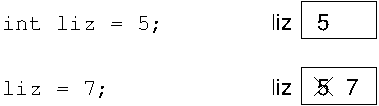
\includegraphics{figs/assign2.pdf}
\end{center}

%TODO(CSM): multiple assignment means "int x=0, y=0;" using the comma operator
%\index{multiple assignment}
%
%\begin{code}
%    int liz = 5;
%    System.out.print(liz);
%    liz = 7;
%    System.out.println(liz);
%\end{code}
%
%The output of this program is {\tt 57}, because the first time we print {\tt liz} her value is 5, and the second time her value is 7.

When there are multiple assignments to a variable, it is especially important to distinguish between an assignment statement and a statement of equality.
Because Java uses the {\tt =} symbol for assignment, it is tempting to interpret a statement like {\tt a = b} as a statement of equality.
It is not!

First of all, equality is commutative, and assignment is not.
For example, in mathematics if $a = 7$ then $7 = a$.
In Java {\tt a = 7;} is a legal assignment statement, but {\tt 7 = a;} is not.
Assignment {\em always} executes from right to left.

Furthermore, in mathematics, a statement of equality is true for all time.
If $a = b$ now, then $a$ will always equal $b$.
In Java, an assignment statement can make two variables equal, but they don't have to stay that way.

\begin{code}
    int a = 5;
    int b = a;     // a and b are now equal
    a = 3;         // a and b are no longer equal
\end{code}

The third line changes the value of {\tt a}, but it does not change the value of {\tt b}, so they are no longer equal.
In some programming languages a different symbol is used for assignment, such as {\tt <-} or {\tt :=}, to avoid this confusion.

%Although multiple assignment is frequently useful, you should use it with caution.
%If the values of variables change often, it can make the code difficult to read and debug.


\section{Relational operators}

\index{operator!relational}
\index{relational operator}
\index{operator!comparison}
\index{comparison operator}

{\bf Relational operators} are used to check conditions like whether two values are equal, or whether one is greater than the other.
The following expressions show how they are used:

\begin{code}
    x == y          // x is equal to y
    x != y          // x is not equal to y
    x > y           // x is greater than y
    x < y           // x is less than y
    x >= y          // x is greater than or equal to y
    x <= y          // x is less than or equal to y
\end{code}

The result of a relational operator is one of two special values, \java{true} or \java{false}.
These values belong to the type \java{boolean}; in fact, they are the only values for the type \java{boolean}.

You are probably familiar with these operations, but notice that the Java syntax is different from mathematical symbols like $=$, $\neq$, and $\le$.
A common error is to use a single \java{=} instead of a double \java{==}.
Remember that \java{=} is the assignment operator, and \java{==} is a comparison operator.
Also, there is no such thing as \java{=<} or \java{=>} operators.

The two sides of a relational operator have to be compatible.
For example, the expression \java{5 < "6"} is invalid because \java{5} is an \java{int} and \java{"6"} is a \java{String}.
When comparing values of different numeric types, Java applies the same conversion rules we saw previously with the assignment operator.
For example, when evaluating the expression \java{5 < 6.0}, Java automatically converts the \java{5} to \java{5.0}.

Most relational operators don't work with strings.
Confusingly, \java{==} and \java{!=} do work with strings---they just don't do what you expect.
We'll explain what they do later; in the meantime, don't use them with strings.
Instead, you should use the \java{String} methods \java{equals} and \java{compareTo}:

\begin{code}
    String fruit1 = "Apple";
    String fruit2 = "Orange";
    System.out.println(fruit1.equals(fruit2));
    System.out.println(fruit1.compareTo(fruit2));
\end{code}


\section{Conditional operators}

\index{conditional operator}
\index{operator!conditional}
\index{logical operator}
\index{operator!logical}

Java has three {\bf conditional operators}: \java{&&}, \java{||}, and \java{!}, which respectively stand for {\it and}, {\it or}, and {\it not}.
The semantics of these operators are similar to their meanings in English.

For example, \java{x > 0 && x < 10} is true when \java{x} is both greater than zero and less than 10.
The expression \java{evenFlag || n \% 3 == 0} is true if {\it either} condition is true, that is, if \java{evenFlag} is true or the number \java{n} is divisible by 3.
Finally, the \java{!} operator inverts a boolean expression.
So \java{!evenFlag} is \java{true} if \java{evenFlag} is \java{false}.

\index{short circuit}

Conditional operators evaluate the second expression only when necessary.
For example, \java{true || anything} is always true, so Java does not need to evaluate the expression \java{anything}.
Likewise, \java{false && anything} is always false.
Ignoring the second operand, when possible, is called {\bf short circuit} evaluation, by analogy with an electrical circuit.
Short circuit evaluation can save time, especially if \java{anything} is a method call.
It can also avoid unnecessary errors, if \java{anything} might fail based on the first operand.

\index{De Morgan's laws}

When solving logic problems using conditional operators, you will often need to negate \java{&&} and \java{||} operations.
{\bf De Morgan's laws} show how to simplify such expressions:

\begin{itemize}
\item \java{!(A && B)} ~is the same as~ \java{!A || !B}
\item \java{!(A || B)} ~is the same as~ \java{!A && !B}
\end{itemize}

In other words, negating a conditional expression is the same as negating each term and changing the operator.
Note that since the \java{!} operator has higher precedence than \java{&&} and \java{||}, you don't need to put parentheses around the individual terms \java{!A} and \java{!B}.

De Morgan's laws also apply to the relational operators.
In this case, negating each term means using the ``opposite'' relational operator.

\begin{itemize}
\item \java{!(x < 5 && y == 3)} ~is the same as~ \java{x >= 5 || y != 3}
\item \java{!(x >= 1 || y != 7)} ~is the same as~ \java{x < 1 && y == 7}
\end{itemize}

It may help to read these examples out loud in English.
For instance, ``If I don't want x to be less than 5, and I don't want y to be 3, then I need x to be greater than or equal to 5, or I need y to be anything but 3.''


\section{DrJava interactions}

A good way to gain experience with relational and conditional operators is to use the Interactions Pane of DrJava.
As shown in Figure~\ref{fig:drjava}, you can declare several variables and {\it interactively} test your logic skills.
Don't forget that you can try out many of the examples in this book this same way.

% try to determine their result before running the code.
%
% ABD: I worry about instructions like this, because students seldom follow them.
% Can we create some exercises (and move this section to the end of the chapter)?

\begin{figure}[!h]
\begin{center}
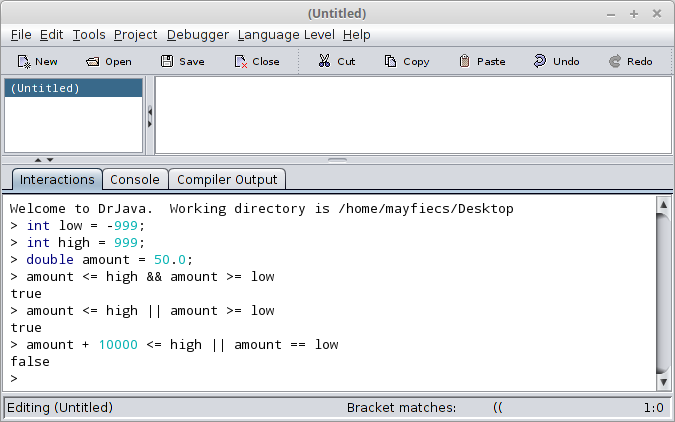
\includegraphics[width=\textwidth]{figs/drjava-logic.png}
\caption{Screenshot of the Interactions Pane in DrJava.}
\label{fig:drjava}
\end{center}
\end{figure}

There is one subtle detail to note when using the Interactions feature.
If you don't end an expression (or statement) with a semicolon, DrJava automatically prints its value.
Notice in Figure~\ref{fig:drjava} how the variable declarations end with semicolons, but the logic expressions in the following lines do not.

What's nice about this feature is that you don't have to create a new class, declare a main method, write arbitrary expressions inside \java{System.out.println} statements, save the source file, and get all of your code to compile in advance.
In addition, you can press the up/down arrows on the keyboard to repeat previous commands and experiment with incremental differences.

\index{order of operations}
\index{precedence}

Notice how none of the expressions in this example require parentheses.
Java evaluates arithmetic operators first, then the relational operators, then conditional operators, and finally the assignment operator.
Do a web search for ``java operator precedence'' to see the complete list of rules.
If two operators have the same precedence, Java evaluates them from left to right.


\section{The if-else statement}

\index{decision statement}
\index{statement!if}

To write useful programs, we almost always need to check conditions and react accordingly.
{\bf Decision statements} give us this ability.
The simplest decision statement in Java is the \java{if} statement:

\begin{code}
    if (x > 0) {
        System.out.println("x is positive");
    }
\end{code}

The expression in parentheses is called the condition.
If it is true, the statements in braces get executed.
If the condition is false, execution skips over that block of code.
The condition in parentheses can be {\it any} boolean expression.

\index{branch}
\index{statement!else}
\index{decision!alternative}

A second form of decision statement is alternative execution, in which there are two possibilities indicated by \java{if} and \java{else}.
The possibilities are called {\bf branches}, and the condition determines which one gets executed:

\begin{code}
    if (x % 2 == 0) {
        System.out.println("x is even");
    } else {
        System.out.println("x is odd");
    }
\end{code}

If the remainder when \java{x} is divided by 2 is zero, we know that \java{x} is even, and this code prints a message to that effect.
If the condition is false, the second print statement is executed instead.
Since the condition must be true or false, exactly one of the alternatives will be executed.

%\label{alternative}
%\index{parity}
%
%To follow up the previous chapter, if you need to check the {\bf parity} (evenness or oddness) of numbers often, you might want to ``wrap'' this code up in a method:
%
%\begin{code}
%    public static void printParity(int x) {
%        if (x % 2 == 0) {
%            System.out.println("x is even");
%        } else {
%            System.out.println("x is odd");
%        }
%    }
%\end{code}
%
%Now you have a method named \java{printParity} that will print an appropriate message for any integer you care to provide.
%In \java{main} you would invoke this method as follows:
%
%\begin{code}
%    printParity(17);
%\end{code}
%
%Always remember that when you invoke a method, you do not have to declare the types of the arguments you provide.
%Java can figure out what type they are.
%You should resist the temptation to write things like:
%
%\begin{code}
%    int number = 17;
%    printParity(int number);        // WRONG!!!
%\end{code}

\index{decision!chained}

Sometimes you want to check related conditions and choose one of several actions.
One way to do this is by {\bf chaining} a series of \java{if} and \java{else} statements:

\begin{code}
    if (x > 0) {
        System.out.println("x is positive");
    } else if (x < 0) {
        System.out.println("x is negative");
    } else {
        System.out.println("x is zero");
    }
\end{code}

These chains can be as long as you want, although they can be difficult to read if they get out of hand.
One way to make them easier to read is to use standard indentation, as demonstrated in these examples.
If you keep all the statements and braces lined up, you are less likely to make syntax errors.

\index{decision!nested}
\index{nested structure}

In addition to chaining, you can also make complex decisions by {\bf nesting} one decision inside another.
We could have written the previous example as:

\begin{code}
    if (x == 0) {
        System.out.println("x is zero");
    } else {
        if (x > 0) {
            System.out.println("x is positive");
        } else {
            System.out.println("x is negative");
        }
    }
\end{code}

The outer conditional has two branches:
the first branch contains a \java{print} statement; the second branch contains another decision statement, which has two branches of its own.
Each of them is a \java{print} statement, but they could have been decision statements as well.

These kinds of nested structures are common, but they get difficult to read very quickly.
Good indentation is essential to make the structure (or intended structure) apparent to the reader.


\section{Flag variables}

\index{expression!boolean}

Recall from Section~\ref{sec:arithops} that an expression is a combination of variables and operators that evaluates to a single value.
Expressions can be as simple as the literal \java{0} or more complex like \java{Math.cos(angle + Math.PI / 2)}.
Boolean expressions and variables work just like other types of expressions and variables:

\begin{code}
    boolean flag;
    flag = true;
    boolean testResult = false;
\end{code}

\index{initialization}
\index{statement!initialization}

The first line is a variable declaration, the second is an assignment, and the third is an initialization.
Since relational operators evaluate to a \java{boolean} value, you can store the result of a comparison in a variable:

\begin{code}
    boolean evenFlag = (n % 2 == 0);    // true if n is even
    boolean positiveFlag = (x > 0);     // true if x is positive
\end{code}

The parentheses are unnecessary, but they make the code easier to read.
A variable defined in this way is called a {\bf flag}, because it signals the presence or absence of some condition.

You can use flag variables as part of a conditional statement later:

\begin{code}
    if (evenFlag) {
        System.out.println("n was even when I checked it");
    }
\end{code}

Notice that you don't need to say \java{if (evenFlag == true)}.
Since \java{evenFlag} is a \java{boolean}, it's already a condition.
Likewise, to check if a flag is \java{false}:

\begin{code}
    if (!evenFlag) {
        System.out.println("n was odd when I checked it");
    }
\end{code}


\section{The return statement}

\index{return}
\index{statement!return}

The \java{return} statement allows you to terminate a method before you reach the end of it.
One reason to use \java{return} is if you detect an error condition:

\begin{code}
    public static void printLogarithm(double x) {
        if (x <= 0.0) {
            System.err.println("Error: x must be positive.");
            return;
        }
        double result = Math.log(x);
        System.out.println("The log of x is " + result);
    }
\end{code}

This example defines a method named \java{printLogarithm} that takes a \java{double} value (named \java{x}) as a parameter.
It checks whether \java{x} is less than or equal to zero, in which case it prints an error message and then uses \java{return} to exit the method.
The flow of execution immediately returns to the caller, and the remaining lines of the method are not executed.

\index{System.err}

Notice the floating-point value \java{0.0} on the right side of the condition.
Since \java{x} is a floating-point variable, you should compare it to a floating-point literal.
This example also uses \java{System.err}, which is the {\it standard error} output stream.
Your development environment might distinguish normal output and error output by using a different color.


\section{Validating input}

Here is a simple program that makes use of the \java{printLogarithm} method defined in the previous section:

\begin{code}
    public static void main(String args[]) {
        Scanner in = new Scanner(System.in);
        System.out.print("Enter a number: ");
        double x = in.nextDouble();
        printLogarithm(x);
    }
\end{code}

Up to this point, we have assumed that users always do what they're told.
But what happens if they make an innocent mistake?
Or even worse, what happens if they deliberately try to crash your program?

\begin{stdout}
Enter a number: Hello
Exception in thread "main" java.util.InputMismatchException
	at java.util.Scanner.throwFor(Scanner.java:909)
	at java.util.Scanner.next(Scanner.java:1530)
	at java.util.Scanner.nextDouble(Scanner.java:2456)
	at Example.main(Example.java:17)
\end{stdout}

In this example, the program calls the \java{nextDouble} method, so the \java{Scanner} attempts to parse a \java{double}.
However the user input is \java{"Hello"}, which causes an \java{InputMismatchException}.
We can prevent this error from happening by checking the input before parsing it:

\begin{code}
    public static void main(String args[]) {
        Scanner in = new Scanner(System.in);
        System.out.print("Enter a number: ");
        if (!in.hasNextDouble()) {
            String word = in.next();
            System.err.println(word + " is not a number");
            return;
        }
        double x = in.nextDouble();
        printLogarithm(x);
    }
\end{code}

The \java{Scanner} class provides \java{hasNext} methods for each of the \java{next} methods.
They return \java{true} or \java{false}, depending on the format of the next token of input.
In this example, we call \java{hasNextDouble} to check if the user entered a \java{double}.
If not, then we display an error message (using \java{System.err}) and abort the program.

If you \java{return} from \java{main}, the program ends immediately.
Notice also the use of the \java{!} operator, instead of the test \java{hasNextDouble() == false}.
Since the \java{hasNextDouble} method returns a boolean result, it is already a condition.


\section{Recursive methods}
\label{recursion}

\index{recursion}

Now that we have methods and if statements, we can explore one of the most magical and interesting things a program can do.
It is common for one method to invoke another, but what happens if a method invokes {\em itself}?
This process is called {\bf recursion}.
Consider the following example:

\begin{code}
    public static void countdown(int n) {
        if (n == 0) {
            System.out.println("Blastoff!");
        } else {
            System.out.println(n);
            countdown(n - 1);
        }
    }
\end{code}

The name of the method is \java{countdown}; it takes a single integer as a parameter.
If the parameter is zero, it prints the word ``Blastoff.''
Otherwise, it prints the number and then invokes itself, passing \java{n - 1} as the argument.

What happens if we invoke \java{countdown(3)} from \java{main}?

\vspace{-1ex}
\begin{quote}
The execution of \java{countdown} begins with \java{n == 3}, and since \java{n} is not zero, it prints the value 3, and then invokes itself...
\begin{quote}
The execution of \java{countdown} begins with \java{n == 2}, and since \java{n} is not zero, it prints the value 2, and then invokes itself...
\begin{quote}
The execution of \java{countdown} begins with \java{n == 1}, and since \java{n} is not zero, it prints the value 1, and then invokes itself...
\begin{quote}
The execution of \java{countdown} begins with \java{n == 0}, and since \java{n} is zero, it prints the word ``Blastoff!'' and then returns.
\end{quote}
The \java{countdown} that got \java{n == 1} returns.
\end{quote}
The \java{countdown} that got \java{n == 2} returns.
\end{quote}
The \java{countdown} that got \java{n == 3} returns.
\end{quote}
\vspace{-1ex}

And then you're back in \java{main}.
So the total output looks like:

\begin{stdout}
3
2
1
Blastoff!
\end{stdout}

As a second example, we'll rewrite the methods \java{newLine} and \java{threeLine} from Section~\ref{adding_methods}.

\begin{code}
    public static void newLine() {
        System.out.println();
    }

    public static void threeLine() {
        newLine();
        newLine();
        newLine();
    }
\end{code}

\index{newline}

Although these methods work, they would not be much help if we wanted to print 2 newlines, or 106.
A better alternative would be:

\begin{code}
    public static void nLines(int n) {
        if (n > 0) {
            System.out.println();
            nLines(n - 1);
        }
    }
\end{code}

This method is similar to \java{countdown}.
As long as $n$ is greater than zero, it prints a newline and then invokes itself to print $(n-1)$ additional newlines.
The total number of newlines is $1 + (n - 1)$, which is just what we wanted: $n$.


\section{Recursive stack diagrams}

\index{stack diagram}
\index{diagram!stack}

In the previous chapter, we used a stack diagram to represent the state of a program during a method invocation.
The same kind of diagram can make it easier to interpret a recursive method.

Remember that every time a method gets called, Java creates a new frame in memory that contains the current method's parameters and variables.
The following figure is a stack diagram for countdown, called with \java{n == 3}:

\begin{figure}[!h]
\begin{center}
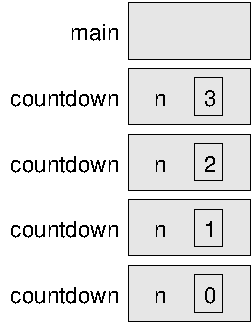
\includegraphics{figs/stack2.pdf}
\caption{Stack diagram for the \java{countdown} program.}
\end{center}
\end{figure}

Note that the ``stack'' of method calls is upside down.
It's easier to draw stack diagrams from top to bottom, because you don't always know how much vertical space you will need in advance.

The stack frame for \java{main} is empty because \java{main} does not have any local variables.
It has one parameter, \java{args}, but since we're not using it, we left it out of the diagram.

There are four frames for \java{countdown}, each with a different value for the parameter \java{n}.
The last frame, with \java{n == 0}, is called the {\bf base case}.
It does not make a recursive call, so there are no more frames below it.

You should always check for a base case in your code, or else the recursion may keep going until the program runs out of memory.
For example, here is a recursive method without a base case:

\begin{code}
    public static void forever(String s) {
        System.out.println(s);
        forever(s); 
    }
\end{code}

\index{call stack}
\index{stack overflow}

This \java{forever} method prints the string over 10,000 times, but then the program suddenly terminates with a \java{StackOverflowError}.
In other words, there's no more room on the stack for additional method calls.

Java sets aside a reasonable amount of memory for the call stack, so that it can remember where to return at the end of each method.
But if that memory fills up, it's usually because you have infinite recursion.

%Recall from Section~\ref{debugger} that Java automatically tracks the call and return of each method in memory, much like the stack diagrams we draw on paper.
%Each method call takes a little memory, but that memory can be reused when the method returns.


\section{Binary Numbers}

The \java{countdown} example has three parts: (1) it checks the base case, (2) prints something, and (3) makes a recursive call.
What do you think happens if you reverse steps 2 and 3, making the recursive call {\it before} printing?

\begin{code}
    public static void countup(int n) {
        if (n == 0) {
            System.out.println("Blastoff!");
        } else {
            countup(n - 1);
            System.out.println(n);
        }
    }
\end{code}

The stack diagram is the same as before, and the method is still called $n$ times.
But now the \java{System.out.println} happens just before each recursive call returns.
As a result, it counts up instead of down:

\begin{stdout}
Blastoff!
1
2
3
\end{stdout}

This behavior comes in handy when it is easier to compute results in reverse order.
For example, to convert a decimal integer into its {\bf binary} representation, you repeatedly divide the number by two:

\begin{stdout}
23 / 2 is 11 remainder 1
11 / 2 is  5 remainder 1
 5 / 2 is  2 remainder 1
 2 / 2 is  1 remainder 0
 1 / 2 is  0 remainder 1
\end{stdout}

So 23 in binary is 10111, which is the remainders in the above example from bottom to top.
Here is a recursive method that prints the binary representation of any positive integer:

\begin{code}
    public static void showBinary(int value) {
        if (value > 0) {
            showBinary(value / 2);
            System.out.print(value % 2);
        }
    }
\end{code}

If \java{value} is zero, \java{showBinary} does nothing (that's the base case).
If the argument is positive, the method divides it by two and calls \java{showBinary} recursively.
When the recursive call returns, the method prints one digit of the result and returns (again).
The leftmost digit is at the bottom of the stack, so it gets printed first.  The rightmost digit, at the top of the stack, gets printed last.

\begin{code}
    showBinary(23);    
    // output is 10111
\end{code}

Learning to think recursively is an important aspect of learning to think like a computer scientist.
Many algorithms can be written concisely with recursive methods that perform computations on the way down, on the way up, or both.


\section{Vocabulary}

\begin{description}

\term{boolean}
A data type with only two values, \java{true} and \java{false}.

\index{operator!relational}
\term{relational operator}
An operator that compares two values and produces a boolean indicating the relationship between them.

\index{operator!conditional}
\term{conditional operator}
An operator that combines boolean values and produces boolean values.

\term{short circuit}
A way of evaluating conditional operators that only evaluates the second operand if necessary.

\term{De Morgan's laws}
Mathematical rules that show how to negate a conditional expression.

\term{decision statement}
A statement that uses a condition to determine which statements to execute.

\term{branch}
One of the alternative sets of statements inside a decision statement.

\term{chaining}
A way of joining several conditional statements in sequence.

\term{nesting}
Putting a conditional statement inside one or both branches of another conditional statement.

\term{flag}
A variable (usually \java{boolean}) that represents a condition or status.

\term{recursion}
The process of invoking the same method that you are currently executing.

\term{base case}
A condition that causes a recursive method {\it not} to make another recursive call.

\term{binary}
A system that uses only zeros and ones to represent numbers.
Also known as ``base 2.''

\end{description}


\section{Exercises}

\begin{exercise}
Conditional operators can simplify nested decision structures.
For example, how can you rewrite this code using a single \java{if} statement?

\begin{code}
    if (x > 0) {
        if (x < 10) {
            System.out.println("x is a positive single digit.");
        }
    }
\end{code}
\end{exercise}

\begin{exercise}
Fermat's Last Theorem says that there are no integers $a$, $b$, and $c$ such that
\[ a^n + b^n = c^n \]
except in the case when $n \leq 2$ (e.g., the Pythagorean Theorem).

Write a method named {\tt checkFermat} that takes four integers as parameters---{\tt a}, {\tt b}, {\tt c} and {\tt n}---and that checks to see if Fermat's theorem holds.
If $n$ is greater than 2 and it turns out to be true that $a^n + b^n = c^n$, the program should print ``Holy smokes, Fermat was wrong!''
Otherwise the program should print ``No, that doesn't work.''

HINT: You may want to use \java{Math.pow} in your method.
\end{exercise}

\begin{exercise}
The purpose of this exercise is to take a problem and break it into smaller problems, and to solve the smaller problems by writing simple methods. Consider the first verse of the song ``99 Bottles of Pop'':

\begin{quote}
99 bottles of pop on the wall,\\
99 bottles of pop,\\
If one of those bottles should happen to fall,\\
98 bottles of pop on the wall.
\end{quote}

Subsequent verses are identical except that the number of bottles gets smaller by one in each verse, until the last verse:

\begin{quote}
1 bottle of pop on the wall,\\
1 bottle of pop,\\
If that last bottle should happen to fall,\\
No more bottles of pop on the wall.
\end{quote}

%And then the song (finally) ends.

Write a program that prints the entire lyrics of ``99 Bottles of Pop.''
Your program should include a {\it recursive} method that does the hard part, but you might want to write additional methods to separate the major functions of the program.
As you develop your code, test it with a small number of verses like ``3 Bottles of Pop.''
\end{exercise}

\begin{exercise}
Draw a stack diagram that shows the state of the program in Section~\ref{recursion} after \java{main} invokes \java{nLines} with the parameter \java{n == 4}, just before the last invocation of \java{nLines} returns.
\end{exercise}

\begin{exercise}
This exercise reviews the flow of execution through a program with multiple methods.
Read the following code and answer the questions.

\begin{code}
public class Buzz {

    public static void baffle(String blimp) {
        System.out.println(blimp);
        zippo("ping", -5);
    }

    public static void zippo(String quince, int flag) {
        if (flag < 0) {
            System.out.println(quince + " zoop");
        } else {
            System.out.println("ik");
            baffle(quince);
            System.out.println("boo-wa-ha-ha");
        }
    }

    public static void main(String[] args) {
        zippo("rattle", 13);
    }

}
\end{code}

\begin{enumerate}

\item Write the number {\tt 1} next to the first {\em statement} of this program that will be executed.
Be careful to distinguish things that are statements from things that are not.

\item Write the number {\tt 2} next to the second statement, and so on until the end of the program.
If a statement is executed more than once, it might end up with more than one number next to it.

\item What is the value of the parameter {\tt blimp} when {\tt baffle} gets invoked?

\item What is the output of this program?

\end{enumerate}
\end{exercise}


\end{document}
